\documentclass{article}
\usepackage{tikz}
\usetikzlibrary{positioning}

\begin{document}

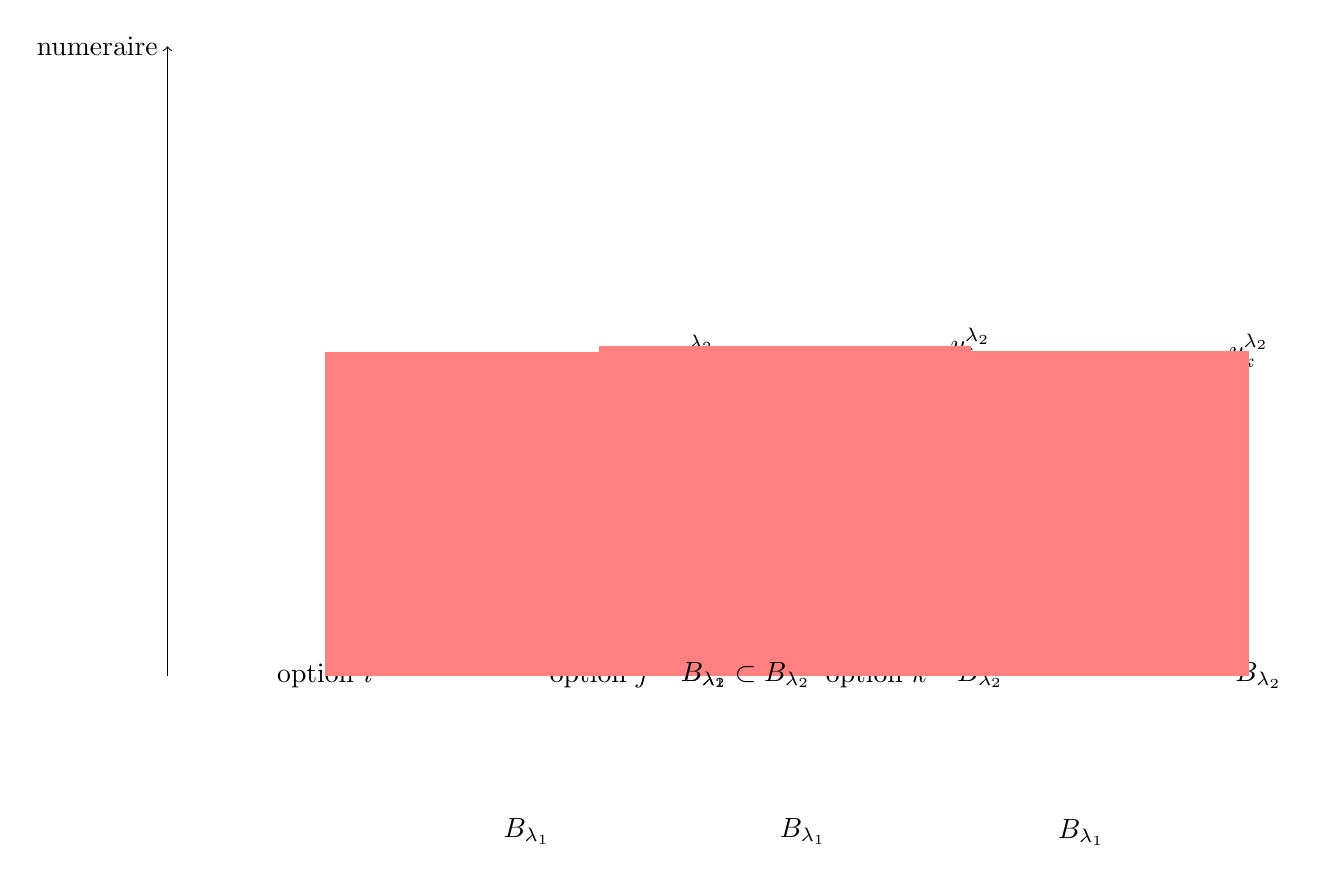
\begin{tikzpicture}[node distance=2cm]
    % Define nodes for the options
    \node (option_i) {option $i$};
    \node[above right=of option_i] (y_i_lambda1) {$y_{i}^{\lambda_{1}}$};
    \node[above right=of y_i_lambda1] (y_i_lambda2) {$y_{i}^{\lambda_{2}}$};
    \node[below right=of option_i] (B_lambda1) {$B_{\lambda_{1}}$};
    \node[above right=of B_lambda1] (B_lambda2) {$B_{\lambda_{2}}$};

    \node[right=of option_i] (option_j) {option $j$};
    \node[above right=of option_j] (y_j_lambda1) {$y_{j}^{\lambda_{1}}$};
    \node[above right=of y_j_lambda1] (y_j_lambda2) {$y_{j}^{\lambda_{2}}$};
    \node[below right=of option_j] (B_lambda1_prime) {$B_{\lambda_{1}}$};
    \node[above right=of B_lambda1_prime] (B_lambda2_prime) {$B_{\lambda_{2}}$};

    \node[right=of option_j] (option_k) {option $k$};
    \node[above right=of option_k] (y_k_lambda1) {$y_{k}^{\lambda_{1}}$};
    \node[above right=of y_k_lambda1] (y_k_lambda2) {$y_{k}^{\lambda_{2}}$};
    \node[below right=of option_k] (B_lambda1_double_prime) {$B_{\lambda_{1}}$};
    \node[above right=of B_lambda1_double_prime] (B_lambda2_double_prime) {$B_{\lambda_{2}}$};

    % Draw the vertical line
    \draw[->] (-2, 0) -- (-2, 8) node[left] {numeraire};

    % Draw the red bars
    \fill[red!50] (option_i) rectangle (y_i_lambda2);
    \fill[red!50] (option_j) rectangle (y_j_lambda2);
    \fill[red!50] (option_k) rectangle (y_k_lambda2);

    % Add the text for the inclusion relation
    \node[above right=of B_lambda1] (inclusion_text) {$B_{\lambda_{1}} \subset B_{\lambda_{2}}$};
\end{tikzpicture}

\end{document}